\chapter{\label{appendix:transformation}Data transformations: Rescaling Data for Display and Analysis}


As fluorescence intensity tends to scale multiplicatively, intensity data needs to be linearised for the purpose of visualisation and clustering.
Clustering algorithms based on variance (average distance to the mean) perform poorly on skewed data.

%Given a finite range (number of channels/bins), a logarithmic transform can be used to maximise the range of data that can be captured by a detector.

Given FCS 2 data is strictly positive, a simple $\log_{10}$ transform is usually applied.
However FCS 3 allows negative values so an offset parameter $b$ may be specified:
\[
    f(x) = \log_{10}(x+b)
\]
However for low and negative intensities, a linear transform is preferred to a logarithmic transform \citep{Tung:2006uw} as it is less distortive.
%this transform distorts the data: it shrinks the distance between points making clusters less distinguishable
Some more appropriate transformations for FCS 3 are the Generalized Arcsinh, the Biexponential, the LinLog and the Generalized BoxCox
\citep{Bagwell:2005he,Parks:2006gaa,Finak:2010is}.
Given the data, parameters for these transformations can be estimated using maximum likelihood assuming a multivariate Gaussian distribution of the data \citep{Finak:2010is}. 

%assume a global distance metric.
%as illustrated in Figure~\ref{figure:transform}.
%One issue in choosing a transform is whether to allow for negative values.
%The simplest transform which can cater for negative values is a log transform with an offset parameter:

% Another possibility is the arcsinh transform which allows for negative values without requiring an offset to be specified:
%\[
    %f(x) = \operatorname{arcsinh}(x) = \log( x^2 + \sqrt { 1+ x^2 } )
%\]

%For the purpose of gating the bead data, the transform chosen for FCS2.0 data is a standard log transform (offset $b=0$)
%whereas for FCS3.0 we use an offset $b=50$ so to make all values positive:
%\[
    %f(x) = log(x+50)
But, as illustrated by \citet{Tung:2006uw}, care needs to be taken in choosing a suitable transform, as the choice of the parameters
infuences the shape of the distribution and can introduce extra modes.
Figure~\ref{figure:log10-transform} illustrates this phenomenon in our data when we apply the $Log_{10}$ transform.
Instead if we apply the logicle transform as defined by \citet{Parks:2006gaa} in Figure~\ref{figure:logicle-transform}, we see that we can address the spurious mode
by reducing the w parameter which influences the slope of the linear transform around zero.

%Update for the Logicle Data Scale Including Operational Code Implementations \citet{Moore:2012gz}

\begin{figure}
\centering
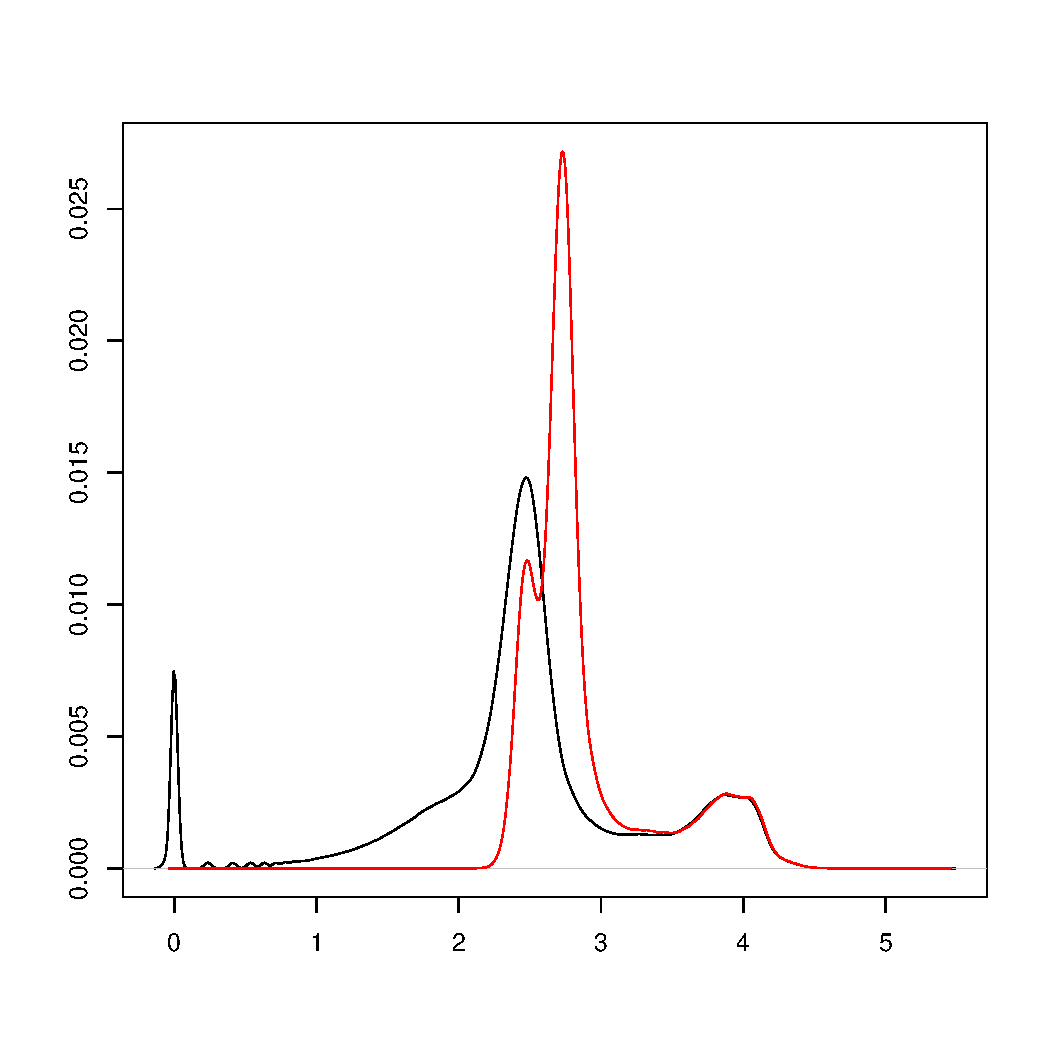
\includegraphics[scale=.5] {Appendix/figures/log10-transform.pdf}
\mycaption{figure:log10-transform} 
{$Log_{10}$ transformed data}
{
  In black, intensity values of zero or less are assigned to zero.
  In red, the intensity value have been shifted by the minimum, before applying the transform, so that all negative values are greater than zero.
}
\end{figure}


\begin{figure}
\centering
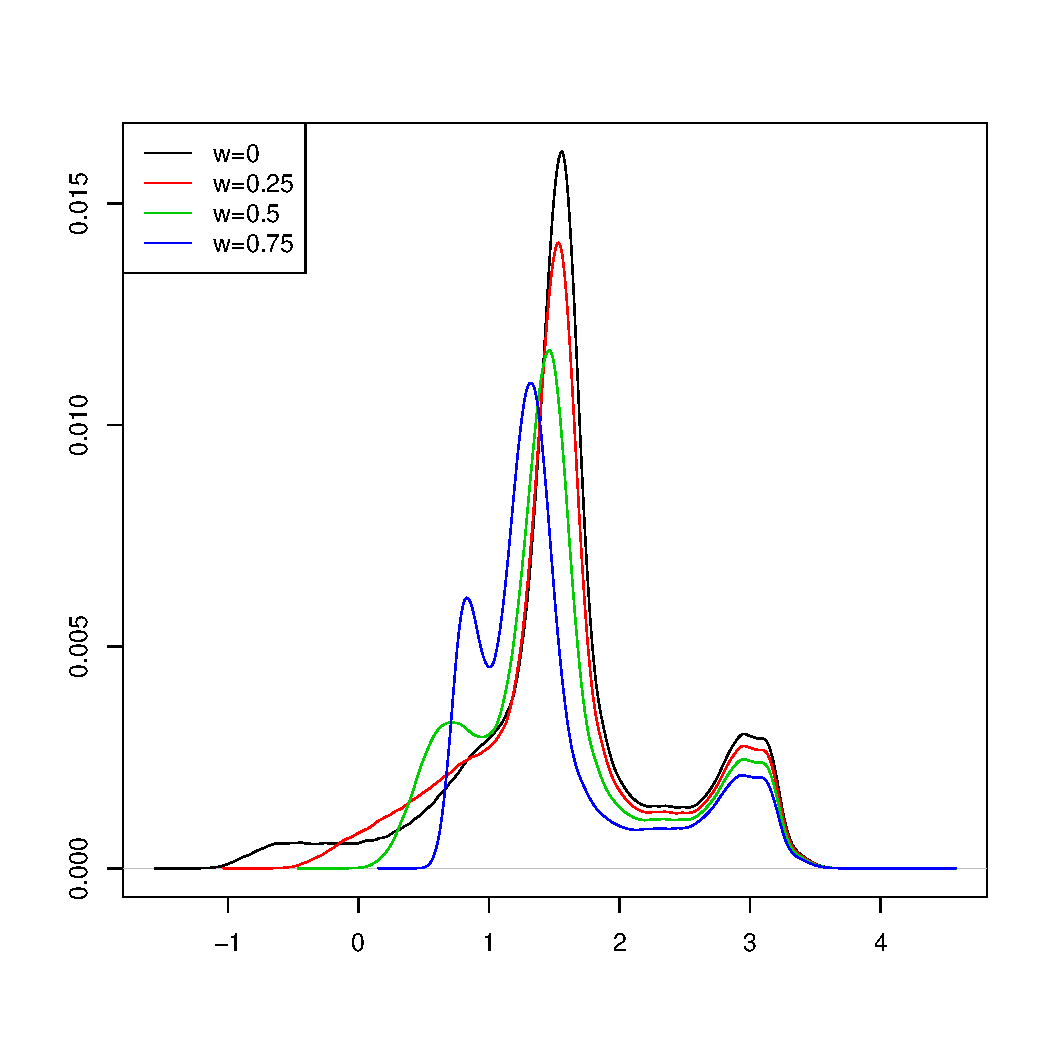
\includegraphics[scale=.5] {Appendix/figures/logicle-transform.pdf}
\mycaption{figure:logicle-transform} 
{$logicle$ transformed data}
{
  The logicle transform is similar to a logistic function in that it approximates a linear transform around the first decade
  and a log transform elsewhere.
  As the slope of the linear transform, increases the shape of the distribution approximates the shifted log transform in Figure~\ref{figure:log10-transform}.
}
\end{figure}


\begin{figure}[ht]
\centering
\begin{subfigure}[b]{.4\textwidth}
    \centering
    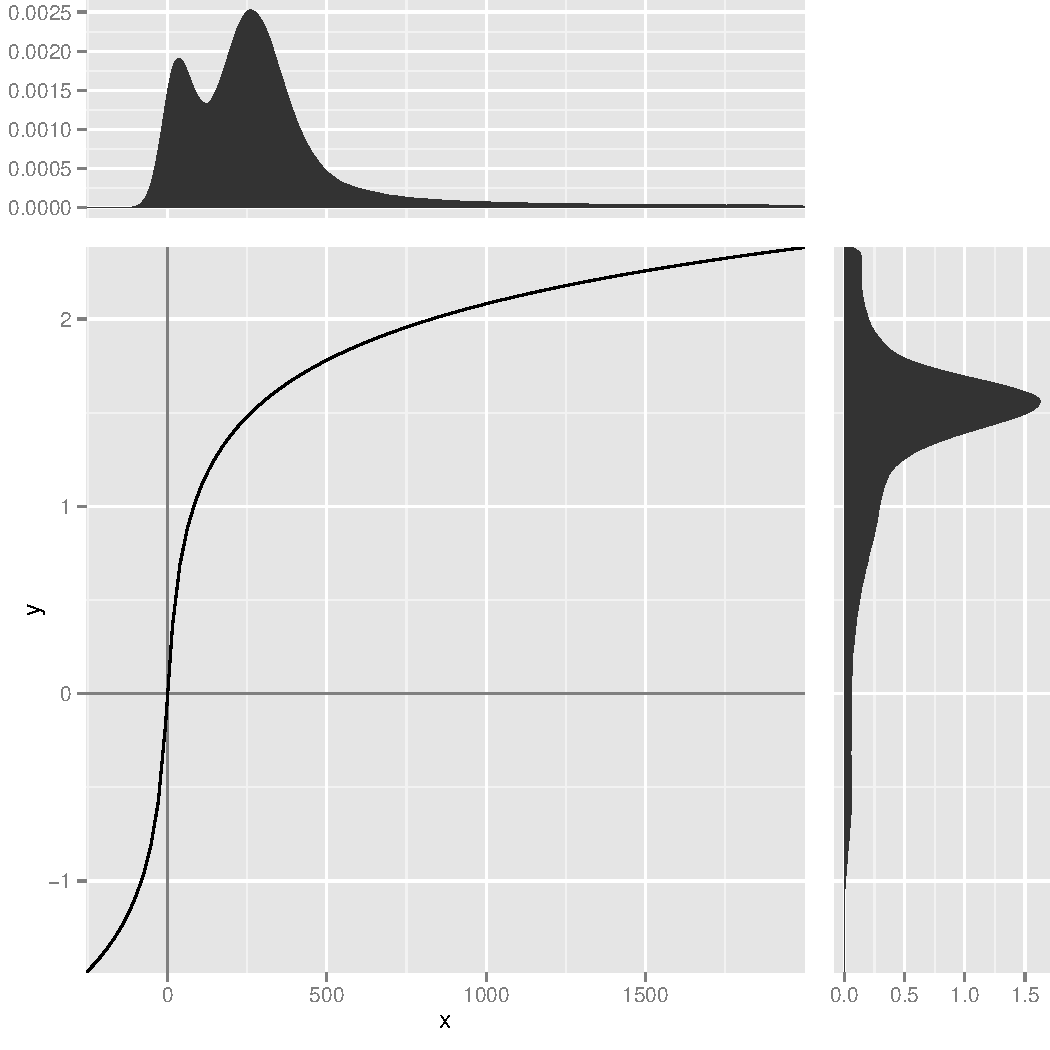
\includegraphics[scale=.3]{Appendix/figures/logicle-transform-a.pdf}
    \caption{w=0}
\end{subfigure}
~
\begin{subfigure}[b]{.4\textwidth}
    \centering
    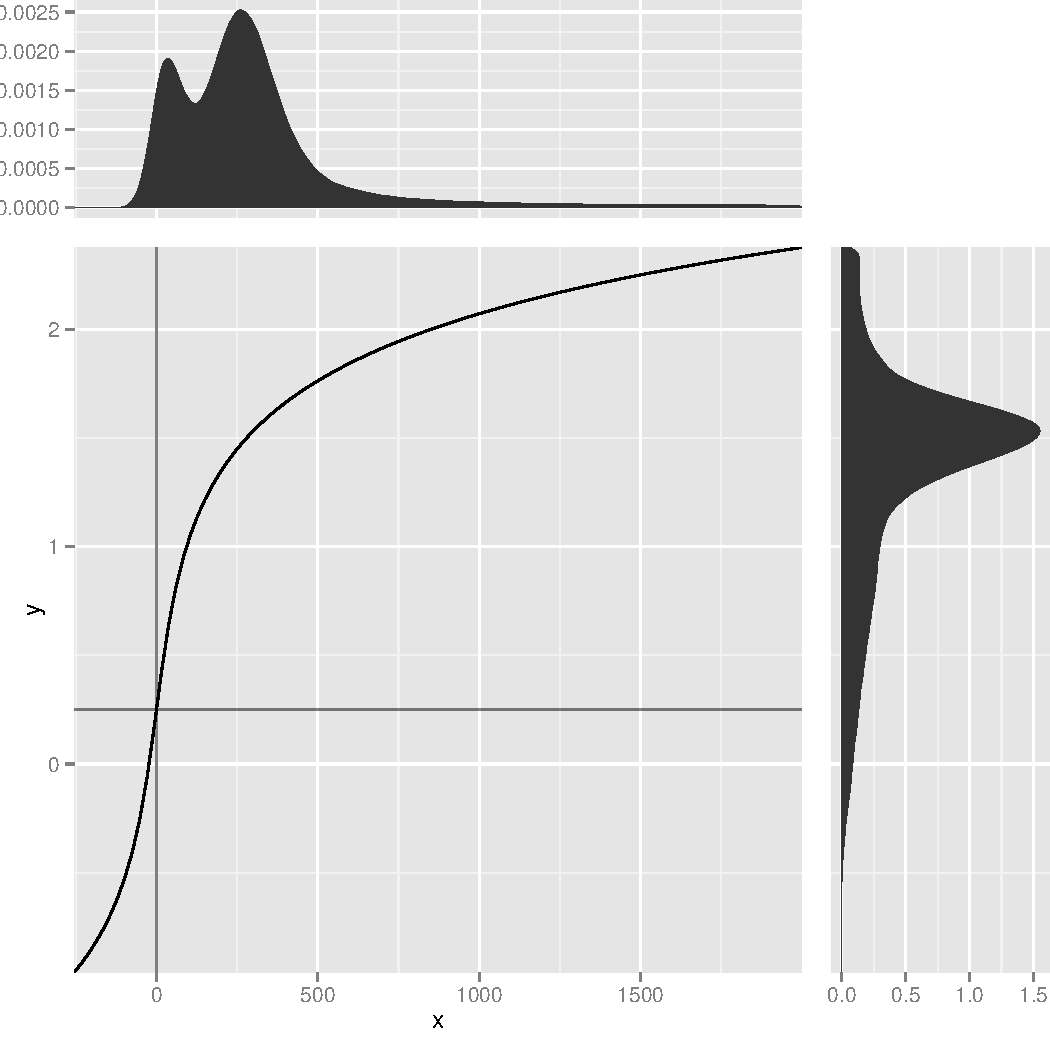
\includegraphics[scale=.3]{Appendix/figures/logicle-transform-b.pdf}
    \caption{w=.25}
\end{subfigure}
~
\begin{subfigure}[b]{.4\textwidth}
    \centering
    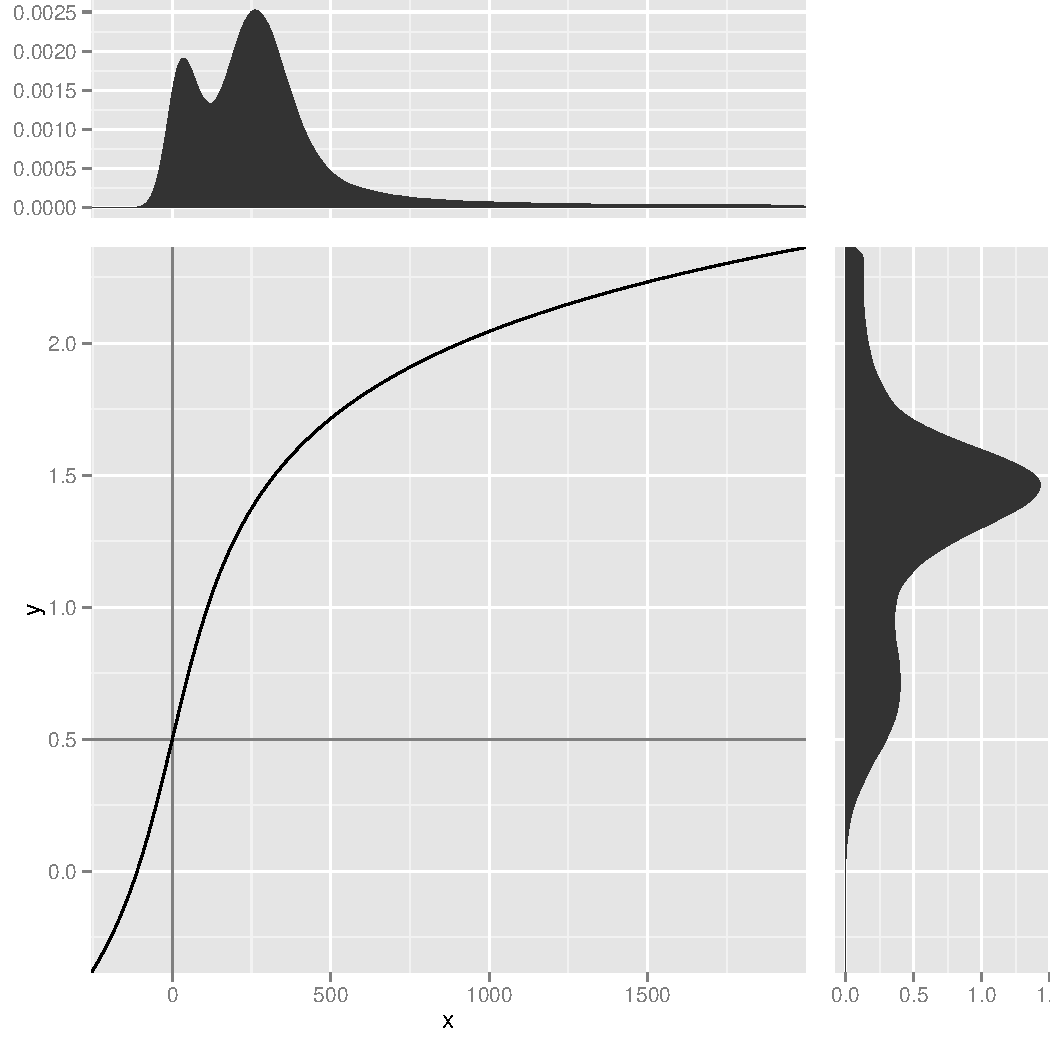
\includegraphics[scale=.3]{Appendix/figures/logicle-transform-c.pdf}
    \caption{w=.5}
\end{subfigure}
~
\begin{subfigure}[b]{.4\textwidth}
    \centering
    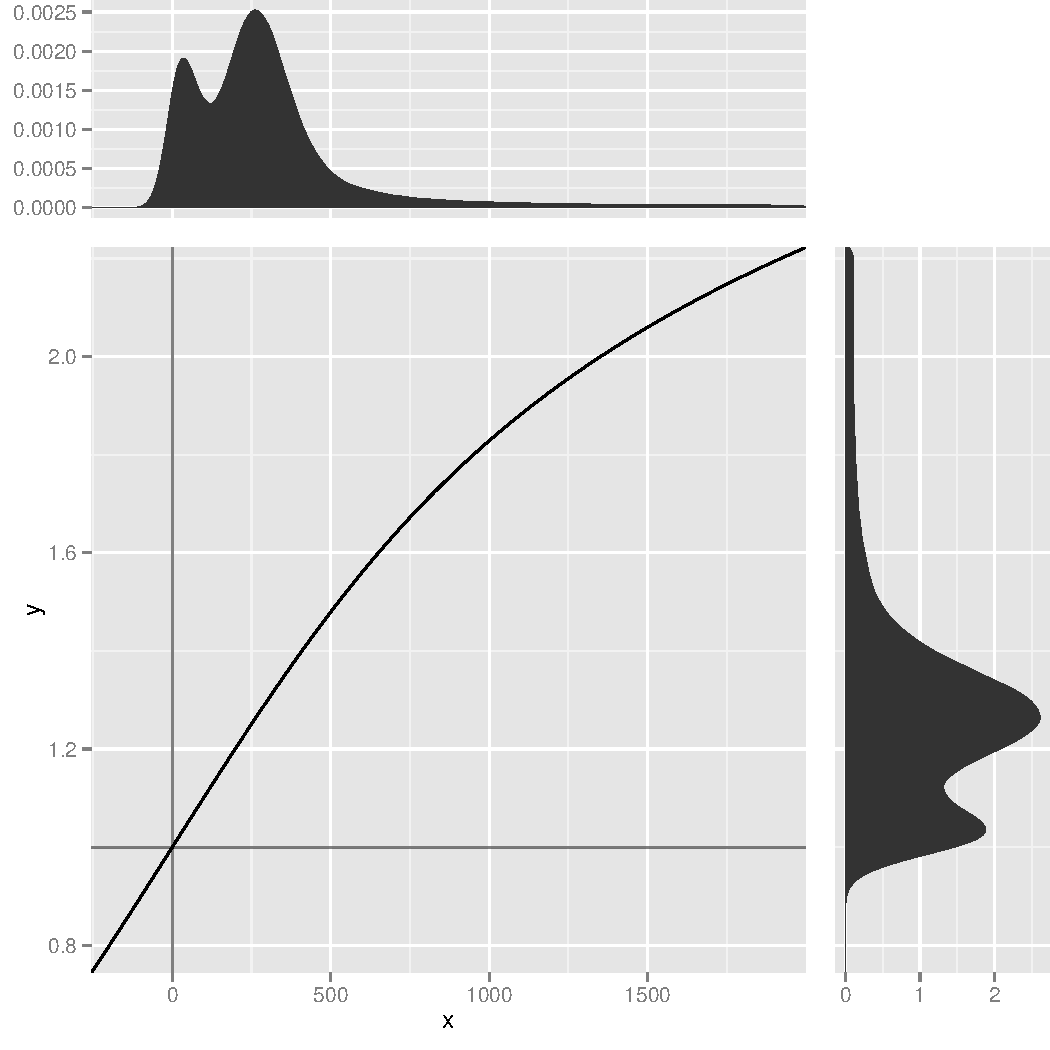
\includegraphics[scale=.3]{Appendix/figures/logicle-transform-d.pdf}
    \caption{w=1}
\end{subfigure}
\mycaption{figure:CD25-MFI-beads-normalised}
{Effect of the w parameter of the logicle transform.}
{
  The w parameter maps the zero of the transform to w.
}
\end{figure}


